\subsection{Instalación de JMeter (Ubuntu)}

Antes de instalar JMeter tenemos que instalar docker y docker-compose para poder descargar el repositorio que se proporciona:

\begin{lstlisting}[language=bash]
    sudo apt-get install docker docker-compose
\end{lstlisting}

Ahora vamos a descargar el repositorio de JMeter proporcionado para hacer la práctica con el siguiente comando:

\begin{figure}[H]
    \centering
    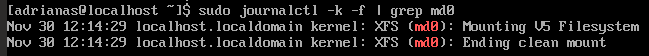
\includegraphics[scale=0.5]{JMeter/img2}
    \caption{Descarga de la carpeta con JMeter}
\end{figure}

Una vez descargada la carpeta, iniciamos el servicio con el comando:

\begin{lstlisting}[language=bash]
    sudo docker-compose up
    sudo docker-compose down
\end{lstlisting}

up para levanatar el servicio y down para pararlo. La ejecución de docker ensucia mucho la pantalla con muchos outputs. Para que no 
que no imprima nada por pantalla, ejecutamos el siguiente comando:

\begin{figure}[H]
    \centering
    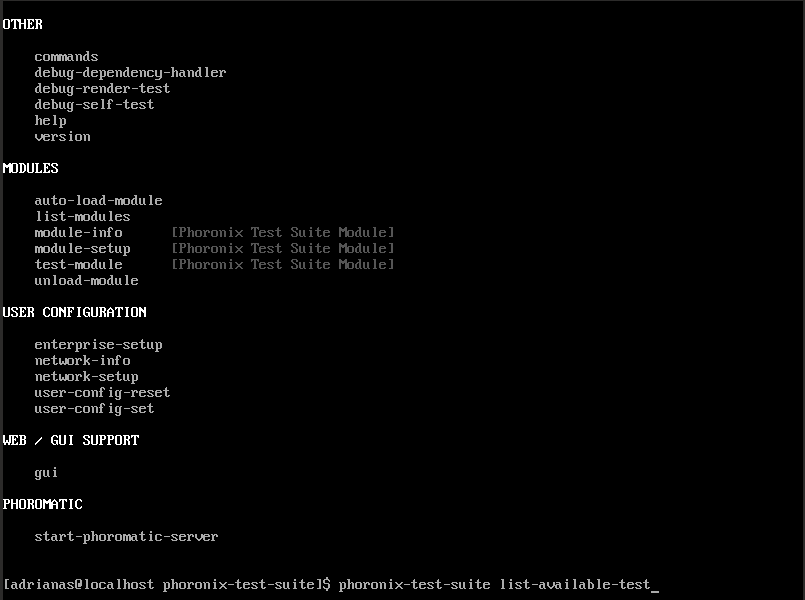
\includegraphics[scale=0.5]{JMeter/img7}
    \caption{Levantar el servicio sin outputs}
\end{figure}

La primera vez tardará un rato ya que tendrá que descargar todos los contenedores. Una vez termine, tendremos que habilitar el puerto 3000 ya que el servicio lo requiere.
Esto, como ya sabemos, lo haremos con el comando:

\begin{lstlisting}[language=bash]
    ufw enable
    ufw allow 3000/tcp    
\end{lstlisting}

Para ver si todo se ha iniciado correctamente, lo comprobamos en un navegador poniendo la IP de nuestro servidor seguido del puerto 3000 y tendría que salir un resultado como el siguiente:

\begin{figure}[H]
    \centering
    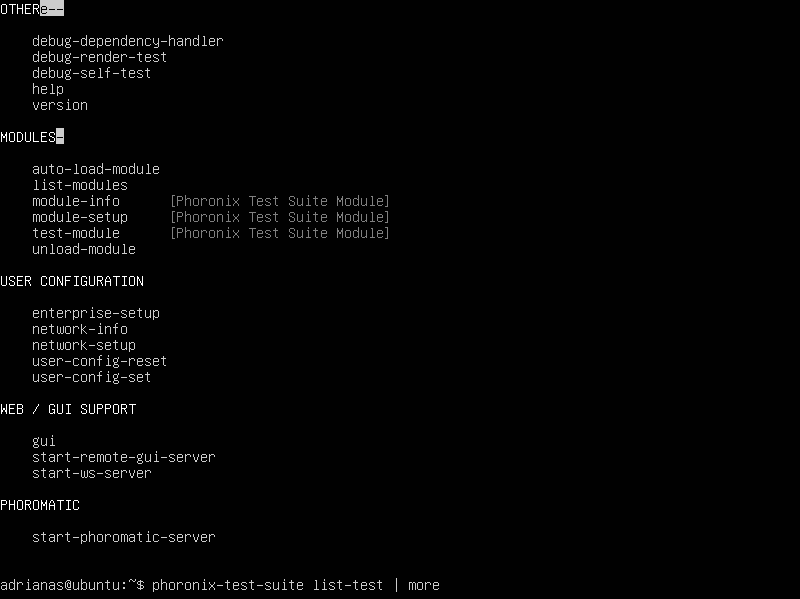
\includegraphics[scale=0.5]{JMeter/img6}
    \caption{Pantalla de inicio del servicio}
\end{figure}

\subsection{Instalación de JMeter en nuestro Host}

El único requisito que tiene JMeter para permitir su ejecución es tener Java instalado y lo podemos comprobar con la ejecución del comando:

\begin{lstlisting}[language=bash]
    java --version
\end{lstlisting}

Una vez tenemos Java instalado, nos vamos a la página oficial de JMeter y lo descargamos. Al descomprimirlo nos vamos a su carpeta y ejecutamos el archivo cuyo nombre es ApacheJMeter.jar

